% Editable standalone vector figure extracted from spectra.tex.
% Source slide 13; figure 13; native embedded fonts.
% Compile with LuaLaTeX from this directory, or run ../export_figures.py.
\documentclass[tikz,border=0pt]{standalone}
% Shared editable preamble for standalone, Nature-style vector figures.
% Text remains embedded and searchable. This is a house-style target, not a
% claim of acceptance or of satisfying every journal's submission checklist.
\usepackage{fontspec}
\setmainfont{LiberationSans}[
  Path=../../shared/assets/,Extension=.ttf,
  UprightFont=*-Regular,BoldFont=*-Bold,ItalicFont=*-Italic,BoldItalicFont=*-BoldItalic]
\setsansfont{LiberationSans}[
  Path=../../shared/assets/,Extension=.ttf,
  UprightFont=*-Regular,BoldFont=*-Bold,ItalicFont=*-Italic,BoldItalicFont=*-BoldItalic]
\setmonofont{LiberationSans}[
  Path=../../shared/assets/,Extension=.ttf,
  UprightFont=*-Regular,BoldFont=*-Bold,ItalicFont=*-Italic,BoldItalicFont=*-BoldItalic]
\usepackage{unicode-math}
\setmathfont{Latin Modern Math}
\DeclareMathSizes{5.9}{6}{5}{5}
\DeclareMathSizes{6}{6}{5}{5}
\usepackage{tikz}
\usetikzlibrary{arrows.meta,calc,positioning,patterns,decorations.pathreplacing,matrix}
\usepackage{graphicx}
\usepackage{xcolor}
\pagecolor{white}
\definecolor{ink}{HTML}{202020}
\definecolor{paper}{HTML}{FFFFFF}
\definecolor{muted}{HTML}{494949}
\definecolor{line}{HTML}{808080}
\definecolor{soft}{HTML}{F0F0F0}
\hyphenpenalty=10000\exhyphenpenalty=10000
\newcommand{\figurefont}{\sffamily\fontsize{5.9}{7.4}\selectfont}
\newcommand{\figuremathfont}{\sffamily\fontsize{6}{7.5}\selectfont}
\newcommand{\brandmedium}{\bfseries}
\renewcommand{\normalsize}{\figurefont}
\renewcommand{\small}{\figurefont}
\renewcommand{\footnotesize}{\figurefont}
\renewcommand{\scriptsize}{\figurefont}
\renewcommand{\tiny}{\figurefont}
\renewcommand{\large}{\figurefont}
\renewcommand{\Large}{\figurefont}
\renewcommand{\LARGE}{\figurefont}
\renewcommand{\huge}{\figurefont}
\renewcommand{\Huge}{\figurefont}
\tikzset{
  every path/.style={line width=.55pt},
  every node/.style={font=\figurefont,text=ink},
  arr/.style={-{Latex[length=1.5mm,width=1mm]},line width=.55pt,draw=ink},
  thinarr/.style={-{Latex[length=1.3mm,width=.9mm]},line width=.55pt,draw=ink},
  box/.style={draw=ink,line width=.55pt,fill=white,minimum height=.85cm,align=center,inner sep=3pt},
  ghost/.style={draw=muted,dashed,fill=soft},
  tag/.style={font=\figurefont,text=muted},
  equ/.style={font=\figuremathfont},
  small/.style={font=\figurefont},
  body/.style={font=\figurefont},
  tinytext/.style={font=\figurefont}
}
\newcommand{\txt}[4]{\node[anchor=north west,align=left,text width=#3cm] at (#1,#2) {#4};}
\newcommand{\smalltxt}[4]{\node[anchor=north west,align=left,text width=#3cm,small] at (#1,#2) {#4};}
\newcommand{\eqn}[4][6]{\node[anchor=north west,font=\figuremathfont] at (#2,#3) {$\displaystyle #4$};}
\newcommand{\diagramblock}[5]{\node[box,minimum width=#3cm,text width=#3cm,minimum height=#4cm] at (#1,#2) {#5};}
% Scale coordinates, not text: all labels retain one final publication size.
\newcommand{\spectrum}[3]{\begin{scope}[shift={(#1,#2)}]
  \draw[muted] (0,0)--({3.6*#3},0);
  \draw[muted] (0,0)--(0,{1.9*#3});
  \foreach \x/\h in {.25/.18,.49/.46,.68/1.42,.87/.37,1.08/.74,1.31/.31,1.57/1.78,1.76/.46,1.96/.19,2.17/1.1,2.37/.57,2.57/.31,2.88/.76,3.21/.23,3.4/.38}{
    \draw[ink] ({\x*#3},0)--({\x*#3},{\h*#3});}
  \foreach \x in {.6,1.2,1.8,2.4,3.0}{\draw[ink] ({\x*#3},0)--+(0,{-.06*#3});}
  \foreach \y in {.45,.9,1.35,1.8}{\draw[ink] (0,{\y*#3})--+({-.06*#3},0);}
  \foreach \x/\lab in {0/0,1.8/45,3.6/90}{\node[anchor=north,font=\figurefont] at ({\x*#3},{-.08*#3}) {\lab};}
  \foreach \y/\lab in {0/0,.9/0.5,1.8/1.0}{\node[anchor=east,font=\figurefont] at ({-.08*#3},{\y*#3}) {\lab};}
  \node[anchor=north east,font=\figurefont] at ({3.6*#3},{-.45*#3}) {$m/z$ (Th)};
  \node[anchor=south west,font=\figurefont] at (0,{1.96*#3}) {Relative intensity (a.u.)};
\end{scope}}
\newcommand{\molecule}[3]{\begin{scope}[shift={(#1,#2)}]
  \draw[ink] (0,{#3})--({.866*#3},{.5*#3})--({.866*#3},{-.5*#3})--(0,{-#3})--({-.866*#3},{-.5*#3})--({-.866*#3},{.5*#3})--cycle;
  \draw[ink] ({.68*#3},{.4*#3})--({.68*#3},{-.4*#3});
  \draw[ink] ({-.7*#3},{-.44*#3})--({-.02*#3},{-.83*#3});
  \draw[ink] ({-.7*#3},{.44*#3})--({-.02*#3},{.83*#3});
  \draw[ink] (0,{#3})--(0,{1.55*#3});
  \node[font=\figurefont] at (0,{1.77*#3}) {OH};
\end{scope}}
\newcommand{\peaktokens}[3]{\foreach \i in {0,...,5}{\pgfmathsetmacro{\xx}{#1+\i*.36}\draw[fill=#3,draw=ink] (\xx,#2) rectangle +(.24,.6);}}
\newcommand{\E}{\mathbb E}
\newcommand{\R}{\mathbb R}
\newcommand{\sg}{\operatorname{stopgrad}}
\newcommand{\LN}{\operatorname{LN}}
\newcommand{\softmax}{\operatorname{softmax}}

\begin{document}
\figurefont
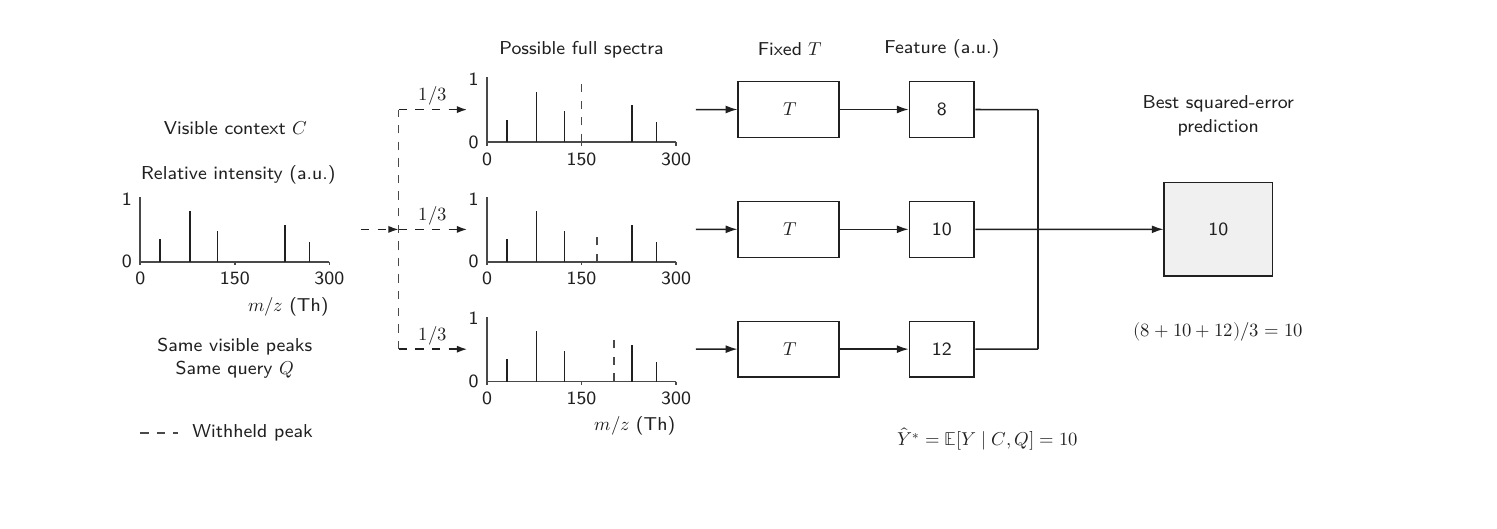
\begin{tikzpicture}[x=1cm,y=1cm,scale=1.14375,transform shape]
% One visible context; no mark, placeholder or mass hint for the withheld peak.
\node[small,inner sep=0] at (2.30,5.74) {Visible context $C$};
\node[tinytext,anchor=west,inner sep=0] at (1.25,5.22) {Relative intensity (a.u.)};
\begin{scope}[shift={(1.25,4.25)}]
 \draw[muted,line width=.55pt] (0,0)--(2.10,0);\draw[muted,line width=.55pt] (0,0)--(0,.72);
 \foreach \x/\h in {.22/.25,.55/.56,.86/.34,1.61/.41,1.88/.22}{\draw[ink,line width=.55pt] (\x,0)--+(0,\h);}
 \foreach \x/\lab in {0/0,1.05/150,2.1/300}{\draw[muted,line width=.55pt] (\x,0)--+(0,-.04);\node[anchor=north,inner sep=1pt,font=\figurefont] at (\x,-.07) {\lab};}
 \foreach \y/\lab in {0/0,.70/1}{\node[anchor=east,inner sep=1pt,font=\figurefont] at (-.05,\y) {\lab};}
 \node[anchor=north east,inner sep=0,tinytext] at (2.10,-.39) {$m/z$ (Th)};
\end{scope}
\node[small,inner sep=0,align=center] at (2.30,3.18) {Same visible peaks\\Same query $Q$};
% Dashed forks denote alternative full inputs, not teacher drift through time.
\draw[thinarr,dashed] (3.70,4.61)--(4.12,4.61);
\draw[muted,dashed,line width=.55pt] (4.12,3.28)--(4.12,5.94);
\node[small,inner sep=0] at (6.15,6.61) {Possible full spectra};
\node[small,inner sep=0] at (8.45,6.61) {Fixed $T$};
\node[small,inner sep=0] at (10.15,6.61) {Feature (a.u.)};
\foreach \base/\hiddenx/\hiddenh/\value/\idx in {5.58/1.05/.65/8/1,4.25/1.22/.31/10/2,2.92/1.41/.48/12/3}{
 \pgfmathsetmacro{\cy}{\base+.36}
 \draw[thinarr,dashed] (4.12,\cy)--node[above,inner sep=1pt,tinytext] {$1/3$}(4.88,\cy);
 \begin{scope}[shift={(5.10,\base)}]
  \draw[muted,line width=.55pt] (0,0)--(2.10,0);\draw[muted,line width=.55pt] (0,0)--(0,.72);
  \foreach \x/\h in {.22/.25,.55/.56,.86/.34,1.61/.41,1.88/.22}{\draw[ink,line width=.55pt] (\x,0)--+(0,\h);}
  \draw[muted,dashed,line width=.55pt] (\hiddenx,0)--+(0,\hiddenh);
  \foreach \x/\lab in {0/0,1.05/150,2.1/300}{\draw[muted,line width=.55pt] (\x,0)--+(0,-.04);\node[anchor=north,inner sep=1pt,font=\figurefont] at (\x,-.07) {\lab};}
  \foreach \y/\lab in {0/0,.70/1}{\node[anchor=east,inner sep=1pt,font=\figurefont] at (-.05,\y) {\lab};}
 \end{scope}
 \node[box,minimum width=1.12cm,minimum height=.62cm,inner sep=3pt] (teacher\idx) at (8.45,\cy) {$T$};
 \draw[arr] (7.42,\cy)--(teacher\idx.west);
 \node[draw=ink,fill=paper,line width=.55pt,minimum width=.72cm,minimum height=.62cm,inner sep=0,font=\figurefont] (feature\idx) at (10.15,\cy) {\value};
 \draw[arr] (teacher\idx.east)--(feature\idx.west);
 \draw[ink,line width=.55pt] (feature\idx.east)--(11.22,\cy);
}
\node[anchor=north east,inner sep=0,tinytext] at (7.20,2.54) {$m/z$ (Th)};
\draw[muted,dashed,line width=.55pt] (1.25,2.35)--(1.67,2.35);
\node[anchor=west,inner sep=0,tinytext] at (1.82,2.35) {Withheld peak};
% A conditional mean: the three teacher outputs are equally probable given C,Q.
\draw[ink,line width=.55pt] (11.22,3.28)--(11.22,5.94);
\node[draw=ink,fill=soft,line width=.55pt,minimum width=1.20cm,minimum height=1.04cm,inner sep=0,font=\figurefont] (bestprediction) at (13.22,4.61) {10};
\draw[arr] (11.22,4.61)--(bestprediction.west);
\node[small,inner sep=0,align=center] at (13.22,5.87) {Best squared-error\\prediction};
\node[inner sep=0,font=\figurefont] at (13.22,3.47) {$(8+10+12)/3=10$};
\node[anchor=west,inner sep=0,font=\figurefont] at (9.65,2.28) {$\widehat Y^*=\mathbb E[Y\mid C,Q]=10$};
% Fixed canvas: 183 x 60.046875 mm. No clipping: overflow is audited.
\pgfresetboundingbox
\path[use as bounding box] (0,1.6) rectangle (16,6.85);
\end{tikzpicture}
\end{document}
